% ****************************************************************************************
% ************************        PRACTICA 1                  ****************************
% ****************************************************************************************


% =======================================================
% =======         HEADER FOR DOCUMENT        ============
% =======================================================
    
    % *********   HEADERS AND FOOTERS ********
    \def\ProjectAuthorLink{https://github.com/CompilandonocimientoCo}           %Just to keep it in line
    \def\ProjectNameLink{\ProjectAuthorLink/Proyect}                %Link to Proyect

    % *********   DOCUMENT ITSELF   **************
    \documentclass[12pt, fleqn]{article}                             %Type of docuemtn and size of font and left eq
    \usepackage[spanish]{babel}                                     %Please use spanish
    \usepackage[utf8]{inputenc}                                     %Please use spanish - UFT
    \usepackage[margin = 1.2in]{geometry}                           %Margins and Geometry pacakge
    \usepackage{ifthen}                                             %Allow simple programming
    \usepackage{hyperref}                                           %Create MetaData for a PDF and LINKS!
    \usepackage{pdfpages}                                           %Create MetaData for a PDF and LINKS!
    \hypersetup{pageanchor = false}                                 %Solve 'double page 1' warnings in build
    \setlength{\parindent}{0pt}                                     %Eliminate ugly indentation
    \author{Laura Andrea Morales López}              %Who I am

    % *********   LANGUAJE    *****************
    \usepackage[T1]{fontenc}                                        %Please use spanish
    \usepackage{textcmds}                                           %Allow us to use quoutes
    \usepackage{changepage}                                         %Allow us to use identate paragraphs
    \usepackage{anyfontsize}                                        %All the sizes

    % *********   MATH AND HIS STYLE  *********
    \usepackage{ntheorem, amsmath, amssymb, amsfonts}               %All fucking math, I want all!
    \usepackage{mathrsfs, mathtools, empheq}                        %All fucking math, I want all!
    \usepackage{cancel}                                             %Negate symbol
    \usepackage{centernot}                                          %Allow me to negate a symbol
    \decimalpoint                                                   %Use decimal point

    % *********   GRAPHICS AND IMAGES *********
    \usepackage{graphicx}                                           %Allow to create graphics
    \usepackage{float}                                              %For images
    \usepackage{wrapfig}                                            %Allow to create images
    \graphicspath{ {Graphics/} }                                    %Where are the images :D

    % *********   LISTS AND TABLES ***********
    \usepackage{listings, listingsutf8}                             %We will be using code here
    \usepackage[inline]{enumitem}                                   %We will need to enumarate
    \usepackage{tasks}                                              %Horizontal lists
    \usepackage{longtable}                                          %Lets make tables awesome
    \usepackage{booktabs}                                           %Lets make tables awesome
    \usepackage{tabularx}                                           %Lets make tables awesome
    \usepackage{multirow}                                           %Lets make tables awesome
    \usepackage{multicol}                                           %Create multicolumns

    % *********   HEADERS AND FOOTERS ********
    \usepackage{fancyhdr}                                           %Lets make awesome headers/footers
    \pagestyle{fancy}                                               %Lets make awesome headers/footers
    \setlength{\headheight}{16pt}                                   %Top line
    \setlength{\parskip}{0.5em}                                     %Top line
    \renewcommand{\footrulewidth}{0.5pt}                            %Bottom line

    \lhead{                                                         %Left Header
        \hyperlink{section.\arabic{section}}                        %Make a link to the current chapter
        {\normalsize{\textsc{\nouppercase{\leftmark}}}}             %And fot it put the name
    }

    \rhead{                                                         %Right Header
        \hyperlink{section.\arabic{section}.\arabic{subsection}}    %Make a link to the current chapter
            {\footnotesize{\textsc{\nouppercase{\rightmark}}}}      %And fot it put the name
    }
    \rfoot{\textsc{\small{\hyperref[sec:Index]{Ve al Índice}}}}     %This will always be a footer  

    \fancyfoot[L]{                                                  %Algoritm for a changing footer
        \ifthenelse{\isodd{\value{page}}}                           %IF ODD PAGE:
            {\href{https://compilandoconocimiento.com/nosotros/}    %DO THIS:
                {\footnotesize                                      %Send the page
                    {\textsc{Laura Andrea Morales López}}}}                 %Send the page
            {\href{https://compilandoconocimiento.com}              %ELSE DO THIS: 
                {\footnotesize                                      %Send the author
                    {\textsc{Practica 1}}}}            %Send the author
    }
    
    
    
% =======================================================
% ===================   COMMANDS    =====================
% =======================================================

    % =========================================
    % =======   NEW ENVIRONMENTS   ============
    % =========================================
    \newenvironment{Indentation}[1][0.75em]                         %Use: \begin{Inde...}[Num]...\end{Inde...}
        {\begin{adjustwidth}{#1}{}}                                 %If you dont put nothing i will use 0.75 em
        {\end{adjustwidth}}                                         %This indentate a paragraph
    \newenvironment{SmallIndentation}[1][0.75em]                    %Use: The same that we upper one, just 
        {\begin{adjustwidth}{#1}{}\begin{footnotesize}}             %footnotesize size of letter by default
        {\end{footnotesize}\end{adjustwidth}}                       %that's it

    \newenvironment{MultiLineEquation}[1]                           %Use: To create MultiLine equations
        {\begin{equation}\begin{alignedat}{#1}}                     %Use: \begin{Multi..}{Num. de Columnas}
        {\end{alignedat}\end{equation}}                             %And.. that's it!
    \newenvironment{MultiLineEquation*}[1]                          %Use: To create MultiLine equations
        {\begin{equation*}\begin{alignedat}{#1}}                    %Use: \begin{Multi..}{Num. de Columnas}
        {\end{alignedat}\end{equation*}}                            %And.. that's it!
    

    % =========================================
    % == GENERAL TEXT & SYMBOLS ENVIRONMENTS ==
    % =========================================
    
    % =====  TEXT  ======================
    \newcommand \Quote {\qq}                                        %Use: \Quote to use quotes
    \newcommand \Over {\overline}                                   %Use: \Bar to use just for short
    \newcommand \ForceNewLine {$\Space$\\}                          %Use it in theorems for example

    % =====  SPACES  ====================
    \DeclareMathOperator \Space {\quad}                             %Use: \Space for a cool mega space
    \DeclareMathOperator \MegaSpace {\quad \quad}                   %Use: \MegaSpace for a cool mega mega space
    \DeclareMathOperator \MiniSpace {\;}                            %Use: \Space for a cool mini space
    
    % =====  MATH TEXT  =================
    \newcommand \Such {\MiniSpace | \MiniSpace}                     %Use: \Such like in sets
    \newcommand \Also {\MiniSpace \text{y} \MiniSpace}              %Use: \Also so it's look cool
    \newcommand \Remember[1]{\Space\text{\scriptsize{#1}}}          %Use: \Remember so it's look cool
    
    % =====  THEOREMS  ==================
    \newtheorem{Theorem}{Teorema}[section]                          %Use: \begin{Theorem}[Name]\label{Nombre}...
    \newtheorem{Corollary}{Colorario}[Theorem]                      %Use: \begin{Corollary}[Name]\label{Nombre}...
    \newtheorem{Lemma}[Theorem]{Lemma}                              %Use: \begin{Lemma}[Name]\label{Nombre}...
    \newtheorem{Definition}{Definición}[section]                    %Use: \begin{Definition}[Name]\label{Nombre}...
    \theoremstyle{break}                                            %THEOREMS START 1 SPACE AFTER

    % =====  LOGIC  =====================
    \newcommand \lIff    {\leftrightarrow}                          %Use: \lIff for logic iff
    \newcommand \lEqual  {\MiniSpace \Leftrightarrow \MiniSpace}    %Use: \lEqual for a logic double arrow
    \newcommand \lInfire {\MiniSpace \Rightarrow \MiniSpace}        %Use: \lInfire for a logic infire
    \newcommand \lLongTo {\longrightarrow}                          %Use: \lLongTo for a long arrow

    % =====  FAMOUS SETS  ===============
    \DeclareMathOperator \Naturals     {\mathbb{N}}                 %Use: \Naturals por Notation
    \DeclareMathOperator \Primes       {\mathbb{P}}                 %Use: \Primes por Notation
    \DeclareMathOperator \Integers     {\mathbb{Z}}                 %Use: \Integers por Notation
    \DeclareMathOperator \Racionals    {\mathbb{Q}}                 %Use: \Racionals por Notation
    \DeclareMathOperator \Reals        {\mathbb{R}}                 %Use: \Reals por Notation
    \DeclareMathOperator \Complexs     {\mathbb{C}}                 %Use: \Complex por Notation
    \DeclareMathOperator \GenericField {\mathbb{F}}                 %Use: \GenericField por Notation
    \DeclareMathOperator \VectorSet    {\mathbb{V}}                 %Use: \VectorSet por Notation
    \DeclareMathOperator \SubVectorSet {\mathbb{W}}                 %Use: \SubVectorSet por Notation
    \DeclareMathOperator \Polynomials  {\mathbb{P}}                 %Use: \Polynomials por Notation
    \DeclareMathOperator \VectorSpace  {\VectorSet_{\GenericField}} %Use: \VectorSpace por Notation
    \DeclareMathOperator \LinealTransformation {\mathcal{T}}        %Use: \LinealTransformation for a cool T
    \DeclareMathOperator \LinTrans {\mathcal{T}}                    %Use: \LinTrans for a cool T


    % =====  CONTAINERS   ===============
    \newcommand{\Set}[1]    {\left\{ \; #1 \; \right\}}             %Use: \Set {Info} for INTELLIGENT space 
    \newcommand{\bigSet}[1] {\big\{  \; #1 \; \big\}}               %Use: \bigSet  {Info} for space 
    \newcommand{\BigSet}[1] {\Big\{  \; #1 \; \Big\}}               %Use: \BigSet  {Info} for space 
    \newcommand{\biggSet}[1]{\bigg\{ \; #1 \; \bigg\}}              %Use: \biggSet {Info} for space 
    \newcommand{\BiggSet}[1]{\Bigg\{ \; #1 \; \Bigg\}}              %Use: \BiggSet {Info} for space 
    
    \newcommand{\Brackets}[1]    {\left[ #1 \right]}                %Use: \Brackets {Info} for INTELLIGENT space
    \newcommand{\bigBrackets}[1] {\big[ \; #1 \; \big]}             %Use: \bigBrackets  {Info} for space 
    \newcommand{\BigBrackets}[1] {\Big[ \; #1 \; \Big]}             %Use: \BigBrackets  {Info} for space 
    \newcommand{\biggBrackets}[1]{\bigg[ \; #1 \; \bigg]}           %Use: \biggBrackets {Info} for space 
    \newcommand{\BiggBrackets}[1]{\Bigg[ \; #1 \; \Bigg]}           %Use: \BiggBrackets {Info} for space 
    
    \newcommand{\Wrap}[1]    {\left( #1 \right)}                    %Use: \Wrap {Info} for INTELLIGENT space
    \newcommand{\bigWrap}[1] {\big( \; #1 \; \big)}                 %Use: \bigBrackets  {Info} for space 
    \newcommand{\BigWrap}[1] {\Big( \; #1 \; \Big)}                 %Use: \BigBrackets  {Info} for space 
    \newcommand{\biggWrap}[1]{\bigg( \; #1 \; \bigg)}               %Use: \biggBrackets {Info} for space 
    \newcommand{\BiggWrap}[1]{\Bigg( \; #1 \; \Bigg)}               %Use: \BiggBrackets {Info} for space 
    
    \newcommand{\Generate}[1]{\left\langle #1 \right\rangle}        %Use: \Wrap {Info} for INTELLIGENT space

    % =====  BETTERS MATH COMMANDS   =====
    \newcommand{\pfrac}[2]{\Wrap{\dfrac{#1}{#2}}}                   %Use: Put fractions in parentesis

    % =========================================
    % ====   LINEAL ALGEBRA & VECTORS    ======
    % =========================================

    % ===== UNIT VECTORS  ================
    \newcommand{\hati} {\hat{\imath}}                               %Use: \hati for unit vector    
    \newcommand{\hatj} {\hat{\jmath}}                               %Use: \hatj for unit vector    
    \newcommand{\hatk} {\hat{k}}                                    %Use: \hatk for unit vector

    % ===== FN LINEAL TRANSFORMATION  ====
    \newcommand{\FnLinTrans}[1]{\mathcal{T}\Wrap{#1}}               %Use: \FnLinTrans for a cool T
    \newcommand{\VecLinTrans}[1]{\mathcal{T}\pVector{#1}}           %Use: \LinTrans for a cool T
    \newcommand{\FnLinealTransformation}[1]{\mathcal{T}\Wrap{#1}}   %Use: \FnLinealTransformation

    % ===== MAGNITUDE  ===================
    \newcommand{\abs}[1]{\left\lvert #1 \right\lvert}               %Use: \abs{expression} for |x|
    \newcommand{\Abs}[1]{\left\lVert #1 \right\lVert}               %Use: \Abs{expression} for ||x||
    \newcommand{\Mag}[1]{\left| #1 \right|}                         %Use: \Mag {Info} 
    
    \newcommand{\bVec}[1]{\mathbf{#1}}                              %Use for bold type of vector
    \newcommand{\lVec}[1]{\overrightarrow{#1}}                      %Use for a long arrow over a vector
    \newcommand{\uVec}[1]{\mathbf{\hat{#1}}}                        %Use: Unitary Vector Example: $\uVec{i}

    % ===== ALL FOR DOT PRODUCT  =========
    \makeatletter                                                   %WTF! IS THIS
    \newcommand*\dotP{\mathpalette\dotP@{.5}}                       %Use: \dotP for dot product
    \newcommand*\dotP@[2] {\mathbin {                               %WTF! IS THIS            
        \vcenter{\hbox{\scalebox{#2}{$\m@th#1\bullet$}}}}           %WTF! IS THIS
    }                                                               %WTF! IS THIS
    \makeatother                                                    %WTF! IS THIS

    % === WRAPPERS FOR COLUMN VECTOR ===
    \newcommand{\pVector}[1]                                        %Use: \pVector {Matrix Notation} use parentesis
        { \ensuremath{\begin{pmatrix}#1\end{pmatrix}} }             %Example: \pVector{a\\b\\c} or \pVector{a&b&c} 
    \newcommand{\lVector}[1]                                        %Use: \lVector {Matrix Notation} use a abs 
        { \ensuremath{\begin{vmatrix}#1\end{vmatrix}} }             %Example: \lVector{a\\b\\c} or \lVector{a&b&c} 
    \newcommand{\bVector}[1]                                        %Use: \bVector {Matrix Notation} use a brackets 
        { \ensuremath{\begin{bmatrix}#1\end{bmatrix}} }             %Example: \bVector{a\\b\\c} or \bVector{a&b&c} 
    \newcommand{\Vector}[1]                                         %Use: \Vector {Matrix Notation} no parentesis
        { \ensuremath{\begin{matrix}#1\end{matrix}} }               %Example: \Vector{a\\b\\c} or \Vector{a&b&c}

    % === MAKE MATRIX BETTER  =========
    \makeatletter                                                   %Example: \begin{matrix}[cc|c]
    \renewcommand*\env@matrix[1][*\c@MaxMatrixCols c] {             %WTF! IS THIS
        \hskip -\arraycolsep                                        %WTF! IS THIS
        \let\@ifnextchar\new@ifnextchar                             %WTF! IS THIS
        \array{#1}                                                  %WTF! IS THIS
    }                                                               %WTF! IS THIS
    \makeatother                                                    %WTF! IS THIS

    % =========================================
    % =======   FAMOUS FUNCTIONS   ============
    % =========================================

    % == TRIGONOMETRIC FUNCTIONS  ====
    \newcommand{\Cos}[1] {\cos\Wrap{#1}}                            %Simple wrappers
    \newcommand{\Sin}[1] {\sin\Wrap{#1}}                            %Simple wrappers
    \newcommand{\Tan}[1] {tan\Wrap{#1}}                             %Simple wrappers
    
    \newcommand{\Sec}[1] {sec\Wrap{#1}}                             %Simple wrappers
    \newcommand{\Csc}[1] {csc\Wrap{#1}}                             %Simple wrappers
    \newcommand{\Cot}[1] {cot\Wrap{#1}}                             %Simple wrappers

    % === COMPLEX ANALYSIS TRIG ======
    \newcommand \Cis[1]  {\Cos{#1} + i \Sin{#1}}                    %Use: \Cis for cos(x) + i sin(x)
    \newcommand \pCis[1] {\Wrap{\Cis{#1}}}                          %Use: \pCis for the same with parantesis
    \newcommand \bCis[1] {\Brackets{\Cis{#1}}}                      %Use: \bCis for the same with Brackets


    % =========================================
    % ===========     CALCULUS     ============
    % =========================================

    % ====== TRANSFORMS =============
    \newcommand{\FourierT}[1]{\mathscr{F} \left\{ #1 \right\} }     %Use: \FourierT {Funtion}
    \newcommand{\InvFourierT}[1]{\mathscr{F}^{-1}\left\{#1\right\}} %Use: \InvFourierT {Funtion}

    % ====== DERIVATIVES ============
    \newcommand \MiniDerivate[1][x] {\dfrac{d}{d #1}}               %Use: \MiniDerivate[var] for simple use [var]
    \newcommand \Derivate[2] {\dfrac{d \; #1}{d #2}}                %Use: \Derivate [f(x)][x]
    \newcommand \MiniUpperDerivate[2] {\dfrac{d^{#2}}{d#1^{#2}}}    %Mini Derivate High Orden Derivate -- [x][pow]
    \newcommand \UpperDerivate[3] {\dfrac{d^{#3} \; #1}{d#2^{#3}}}  %Complete High Orden Derivate -- [f(x)][x][pow]
    
    \newcommand \MiniPartial[1][x] {\dfrac{\partial}{\partial #1}}  %Use: \MiniDerivate for simple use [var]
    \newcommand \Partial[2] {\dfrac{\partial \; #1}{\partial #2}}   %Complete Partial Derivate -- [f(x)][x]
    \newcommand \MiniUpperPartial[2]                                %Mini Derivate High Orden Derivate -- [x][pow] 
        {\dfrac{\partial^{#2}}{\partial #1^{#2}}}                   %Mini Derivate High Orden Derivate
    \newcommand \UpperPartial[3]                                    %Complete High Orden Derivate -- [f(x)][x][pow]
        {\dfrac{\partial^{#3} \; #1}{\partial#2^{#3}}}              %Use: \UpperDerivate for simple use

    \DeclareMathOperator \Evaluate  {\Big|}                         %Use: \Evaluate por Notation

    % =========================================
    % ========    GENERAL STYLE     ===========
    % =========================================
    
    % =====  COLORS ==================
    \definecolor{RedMD}{HTML}{F44336}                               %Use: Color :D        
    \definecolor{Red100MD}{HTML}{FFCDD2}                            %Use: Color :D        
    \definecolor{Red200MD}{HTML}{EF9A9A}                            %Use: Color :D        
    \definecolor{Red300MD}{HTML}{E57373}                            %Use: Color :D        
    \definecolor{Red700MD}{HTML}{D32F2F}                            %Use: Color :D 

    \definecolor{PurpleMD}{HTML}{9C27B0}                            %Use: Color :D        
    \definecolor{Purple100MD}{HTML}{E1BEE7}                         %Use: Color :D        
    \definecolor{Purple200MD}{HTML}{EF9A9A}                         %Use: Color :D        
    \definecolor{Purple300MD}{HTML}{BA68C8}                         %Use: Color :D        
    \definecolor{Purple700MD}{HTML}{7B1FA2}                         %Use: Color :D 

    \definecolor{IndigoMD}{HTML}{3F51B5}                            %Use: Color :D        
    \definecolor{Indigo100MD}{HTML}{C5CAE9}                         %Use: Color :D        
    \definecolor{Indigo200MD}{HTML}{9FA8DA}                         %Use: Color :D        
    \definecolor{Indigo300MD}{HTML}{7986CB}                         %Use: Color :D        
    \definecolor{Indigo700MD}{HTML}{303F9F}                         %Use: Color :D 

    \definecolor{BlueMD}{HTML}{2196F3}                              %Use: Color :D        
    \definecolor{Blue100MD}{HTML}{BBDEFB}                           %Use: Color :D        
    \definecolor{Blue200MD}{HTML}{90CAF9}                           %Use: Color :D        
    \definecolor{Blue300MD}{HTML}{64B5F6}                           %Use: Color :D        
    \definecolor{Blue700MD}{HTML}{1976D2}                           %Use: Color :D        
    \definecolor{Blue900MD}{HTML}{0D47A1}                           %Use: Color :D  

    \definecolor{CyanMD}{HTML}{00BCD4}                              %Use: Color :D        
    \definecolor{Cyan100MD}{HTML}{B2EBF2}                           %Use: Color :D        
    \definecolor{Cyan200MD}{HTML}{80DEEA}                           %Use: Color :D        
    \definecolor{Cyan300MD}{HTML}{4DD0E1}                           %Use: Color :D        
    \definecolor{Cyan700MD}{HTML}{0097A7}                           %Use: Color :D        
    \definecolor{Cyan900MD}{HTML}{006064}                           %Use: Color :D 

    \definecolor{TealMD}{HTML}{009688}                              %Use: Color :D        
    \definecolor{Teal100MD}{HTML}{B2DFDB}                           %Use: Color :D        
    \definecolor{Teal200MD}{HTML}{80CBC4}                           %Use: Color :D        
    \definecolor{Teal300MD}{HTML}{4DB6AC}                           %Use: Color :D        
    \definecolor{Teal700MD}{HTML}{00796B}                           %Use: Color :D        
    \definecolor{Teal900MD}{HTML}{004D40}                           %Use: Color :D 

    \definecolor{GreenMD}{HTML}{4CAF50}                             %Use: Color :D        
    \definecolor{Green100MD}{HTML}{C8E6C9}                          %Use: Color :D        
    \definecolor{Green200MD}{HTML}{A5D6A7}                          %Use: Color :D        
    \definecolor{Green300MD}{HTML}{81C784}                          %Use: Color :D        
    \definecolor{Green700MD}{HTML}{388E3C}                          %Use: Color :D        
    \definecolor{Green900MD}{HTML}{1B5E20}                          %Use: Color :D

    \definecolor{AmberMD}{HTML}{FFC107}                             %Use: Color :D        
    \definecolor{Amber100MD}{HTML}{FFECB3}                          %Use: Color :D        
    \definecolor{Amber200MD}{HTML}{FFE082}                          %Use: Color :D        
    \definecolor{Amber300MD}{HTML}{FFD54F}                          %Use: Color :D        
    \definecolor{Amber700MD}{HTML}{FFA000}                          %Use: Color :D        
    \definecolor{Amber900MD}{HTML}{FF6F00}                          %Use: Color :D

    \definecolor{BlueGreyMD}{HTML}{607D8B}                          %Use: Color :D        
    \definecolor{BlueGrey100MD}{HTML}{CFD8DC}                       %Use: Color :D        
    \definecolor{BlueGrey200MD}{HTML}{B0BEC5}                       %Use: Color :D        
    \definecolor{BlueGrey300MD}{HTML}{90A4AE}                       %Use: Color :D        
    \definecolor{BlueGrey700MD}{HTML}{455A64}                       %Use: Color :D        
    \definecolor{BlueGrey900MD}{HTML}{263238}                       %Use: Color :D        

    \definecolor{DeepPurpleMD}{HTML}{673AB7}                        %Use: Color :D

    \newcommand{\Color}[2]{\textcolor{#1}{#2}}                      %Simple color environment
    \newenvironment{ColorText}[1]                                   %Use: \begin{ColorText}
        { \leavevmode\color{#1}\ignorespaces }                      %That's is!

    % =====  CODE EDITOR =============
    \lstdefinestyle{CompilandoStyle} {                              %This is Code Style
        backgroundcolor     = \color{BlueGrey900MD},                %Background Color  
        basicstyle          = \tiny\color{white},                   %Style of text
        commentstyle        = \color{BlueGrey200MD},                %Comment style
        stringstyle         = \color{Green300MD},                   %String style
        keywordstyle        = \color{Blue300MD},                    %keywords style
        numberstyle         = \tiny\color{TealMD},                  %Size of a number
        frame               = shadowbox,                            %Adds a frame around the code
        breakatwhitespace   = true,                                 %Style   
        breaklines          = true,                                 %Style   
        showstringspaces    = false,                                %Hate those spaces                  
        breaklines          = true,                                 %Style                   
        keepspaces          = true,                                 %Style                   
        numbers             = left,                                 %Style                   
        numbersep           = 10pt,                                 %Style 
        xleftmargin         = \parindent,                           %Style 
        tabsize             = 4,                                    %Style
        inputencoding       = utf8/latin1                           %Allow me to use special chars
    }
 
    \lstset{style = CompilandoStyle}                                %Use this style


    % =========================================
    % =======   ALAN THINGS ===================
    % =========================================

\lstdefinestyle{customc}{
    belowcaptionskip=1\baselineskip,
    breaklines=true,
    frame=L,
    xleftmargin=\parindent,
    language=C,
    showstringspaces=false,
    basicstyle=\ttfamily,
    keywordstyle=\bfseries\color{green!40!black},
    commentstyle=\itshape\color{purple!40!black},
    identifierstyle=\color{blue},
    numbers=left,
    stringstyle=\color{orange},
}

\lstset{escapechar=@,style=customc,tabsize=4,language=C}
%\usepackage{minted}
\usepackage{pgfplots}
\usepackage{xcolor}
\usepackage{tablefootnote}
\usepackage[toc,page]{appendix}

\usepackage{algpseudocode}
\usepackage{algorithm}


\addto\captionsspanish{%
	\renewcommand\appendixname{Anexo}
	\renewcommand\appendixpagename{Anexos}
}
\setlength{\headheight}{15pt} 
\renewcommand{\footrulewidth}{0.5pt}
\setlength{\parskip}{0.5em}



\title{Práctica 1: Calculadora de IP}
\author{3CM3\\
	ESCOM-IPN}


%%%%%%%%%%%%%%%%%%%%%%%%        LALA THINGS     %%%%%%%%%%%%%%%%%%%%%%%%%
\pgfplotsset{compat=1.13}
\usepackage{listings}




\bibliographystyle{IEEEtran}
\begin{document}
\begin{titlepage}
    
    % ============ TITLE PAGE STYLE  ================
    \definecolor{TitlePageColor}{cmyk}{1,.60,0,.40}                 %Simple colors
    \definecolor{ColorSubtext}{cmyk}{1,.50,0,.10}                   %Simple colors
    \newgeometry{left=0.20\textwidth}                               %Defines an Offset
    \pagecolor{TitlePageColor}                                      %Make it this Color to page
    \color{white}                                                   %General things should be white

    % ===== MAKE SOME SPACE =========
    \vspace                                                         %Give some space
    \baselineskip                                                   %But we need this to up command

    % ============ NAME OF THE PROJECT  ============
    \makebox[0pt][l]{\rule{1.3\textwidth}{3pt}}                     %Make a cool line
    
    \href{https://compilandoconocimiento.com}                       %Link to project
    {\textbf{\textsc{\Huge ESCOM-IPN}}}\\[2.7cm]                    %Name of project   

    % ============ NAME OF THE BOOK  ===============
    \href{\ProjectNameLink/LibroRedes}                       %Link to Author
    {\fontsize{36}{50}                                              %Size of the book
        \selectfont \textbf{Ejercicio 2}}\\[0.5cm]       %Name of the book
    {\fontsize{36}{50}                                              %Size of the book
        \selectfont \textbf{Análisis de Complejidad}}\\[0.5cm]                %Name of the book
    \textcolor{ColorSubtext}                                        %Color or the topic
        {\textsc{\LARGE Análisis de Algoritmos}}     %Name of the general theme
    
    \vfill                                                          %Fill the space
    
    % ============ NAME OF THE AUTHOR  =============
    \href{https://compilandoconocimiento.com/}                    %Link to Author
    {\LARGE \textsf{Laura Andrea Morales López}}   %Author

    % ===== MAKE SOME SPACE =========
    \vspace                                                         %Give some space
    \baselineskip                                                   %But we need this to up command
    
    {\large \textsf{Marzo 2018}}                                  %Date

    %%%%%%%%%%%%%%%%%%%%%%%%%%%%%%%%%%%%%%%%%%%%%%%%%%%%%%%%%%%%%%%%%%
    %%%%%%%%%%%%%%%%%   ABSTRACT    %%%%%%%%%%%%%%%%%%%%%%%%%%%%%%%%%%
   
    \begin{figure}[H]
               \centering
                
\includegraphics[scale=.3]{Laura.jpg}
            \end{figure}
\end{titlepage}


% =====================================================
% ==========      RESTORE TO DOCUMENT      ============
% =====================================================
\restoregeometry                                                    %Restores the geometry
\nopagecolor                                                        %Use to restore the color to white




% =====================================================
% ========                INDICE              =========
% =====================================================
\tableofcontents{}
\label{sec:Index}

\clearpage
% =====================================================
%==========         INTRODUCCION            ===========
%======================================================

\section{Complejidad temporal y espacial}
    \subsection{Algoritmo 1:}
    \lstinputlisting[language=C]{1.c}

    Tenemos 2 ciclos que analizar.

    El for que se encuentra mas dentro tiene 5 instrucciones, 2 asignaciones y 2 operaciones. 

    Dentro del for tenemos una resta y una suma.

    Y el n sería $n-2$ pues hay una restriccion de que debe ser menor que $n-1$.

    Entonces, tenemos un bloque de 5 instrucciones que se repiten $n-2$ veces y luego una comparacion una resta y una suma y asignación dentro de la definicion que se repiten $n-2$ veces, un salto que se repite $n-2$, una asignacion al inicio una ultima comparación, una ultima resta y un salto cuando en for no entra en el ciclo.

    Tenemos lo siguiente:

    $5(n-2)+4(n-2)+(n-2)+4$

    $10(n-2)+4$

    $10n-6$

    Después tenemos el siguiente for que es una asignacion al inicio una comparación $n-1$ veces, una asignación, suma y salto implicito $n-1$veces y una comparación final con salto final.
    Para este for tenemos la complejidad.


    $4(n-1)+3$


    Y colocamos la complejidad del anterior, entonces:

    $(10n-6+4)(n-1)+3$


    La complejidad de este algoritmo es $10n^{2}-12n+5$

    La complejidad espacial es el tamaño del arreglo 2 iteradores y la variable temp.

    La complejidad espacial es: $n+3$

    \subsection{Algoritmo 2:}
    \lstinputlisting[language=C]{2.c}

    Tenemos una asignación al principio de este algoritmo
    y tenemos 3 operaciones detro del for con una asignación.

    En el for tenemos una asignacion inicial, una comparación final y un salto.

    Tenemos una comparación, una suma, una asignación y un salto $n+1$ veces

    $8(n+1)+4$

    La complejidad de este algoritmo es $8n+12$

    La complejidad espacial sería el tamaño del Arreglo, el iterador y la variable.

    La complejidad espacial es:$n+3$

    \subsection{Algoritmo 3:}
    \lstinputlisting[language=C]{3.c}
    El for más adentro: 

    Tiene 1 asignación y 2 operaciones.
    Tiene en su definicion tiene una comparación, una asignacion y suma y un salto. Todo esto $n$ veces.

    Tiene una asignación inicial, una compaacion final y un salto final.

    Su complejidad es $7n+3$

    Para el siguiente for tenemos:

    Una asignación,una comparación, una suma, una asignación y un salto $n$ veces.

    Tiene una asignación inicial, una compaacion final y un salto final.

    Entonces colocandolo con el anterior tenemos:

    $(7n+3+5)(n)+3$

    $7n^{2}+8n+3$

    Finalmente para el ultimo ciclo tenemos:

    Una comparación, una suma, una asignación y un salto $n$ veces.

    Tiene una asignación inicial, una compaacion final y un salto final.

    Con el demás algoritmo tenemos

    $(7n^{2}+8n+3+4)(n)+3$

    La complejidad de este algoritmo es:$7n^{3}+8n^{2}+7n+3$

    La complejidad espacial esta dada por las 3 matrices $n^{2}$ y los 3 iteradores$=3n^{2}+3$

    \subsection{Algoritmo 4:}
    \lstinputlisting[language=C]{4.c}
    Para este algoritmo tenemos un while:

    Dentro del while tenemos 6 instrucciones que se repetiran $n-2$ veces.

    Ademas tenemos el salto y la comparacion que igual serán realizadas $n-2$ veces.

    Dos asignaciones iniciales.

    Tenemos $6(n-2)+2(n-2)+2$

    La complejidad de este algoritmo es $8n-14$.
    La complejidad espacial s solo las tres variables=$3$

    \subsection{Algoritmo 5:}

    \lstinputlisting[language=C]{5.c}

    En este algoritmo tenemos dentro del for 2 asignaciones y una operación inicial ademas del salto final y la comparacion final.

    Una comparacion, tres asignaciones,y 2 operaciones, además del salto esto $n$ veces.

    La complejidadsería de $7n+5$.

    La del segundo for seria una asignacion inicial, un salto final y una comparacion final.

    Una asignación, un salto,una comparacion, una suma y una 
    asignacion $n$ veces.Entonces es $=5n+3$

    Entonces nuestra complejidad total es $=12n+8$

    La complejidad espacial es el tamaño de los 2 arreglos mas los 2 iteradores. $=2n+2$
    \section{Impresiones}
    \subsection{Algoritmo 6:}

    \lstinputlisting[language=C]{6.c}
    Notemos que i no puede ser 0, entonces sabemos que cambia respecto al parameto inicial y la iteración es una multiplicación. Se comporta como una progresión geometrica donde $i=10(2)^{k-1}$

    Entonces debe mantenerse en medio de los limites $10<=10(2)^{k-1}<=5n$ Tenemos que $1<=k<=log_{2}\dfrac{5n}{10}+1$

    Asi tenemos que $= log_{2}\dfrac{5n}{10} +1$ será el numero de prints que tendremos.

    Para n=10 tendremos un número de impresiones =3.

    Para n=100 tendremos un número de impresiones =6.

    Para n=1000 tendremos un número de impresiones =9.

    Para n=5000 tendremos un número de impresiones =12.

    Para n=100000 tendremos un número de impresiones =16.

    \subsubsection{Pruebas}
    \lstinputlisting[language=C]{6P.c}
    \begin{figure}[H]
               \centering
                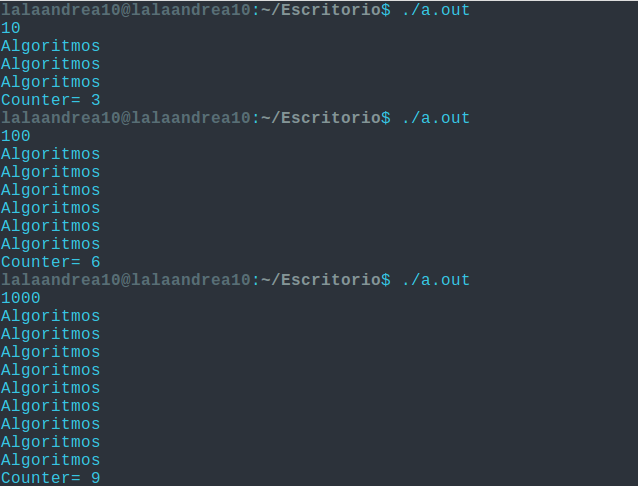
\includegraphics[scale=.5]{10-1000.png}
            \end{figure}

    \begin{figure}[H]
               \centering
                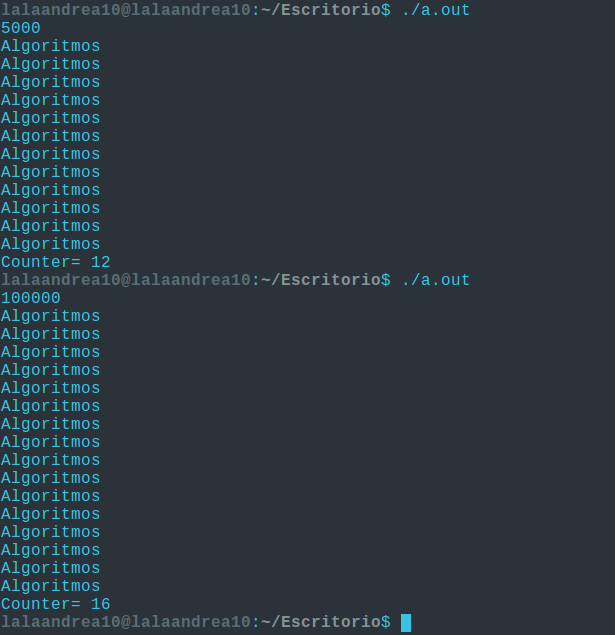
\includegraphics[scale=.5]{5000.png}
            \end{figure}

    \subsection{Algoritmo 7:}
    \lstinputlisting[language=C]{7.c}
    El for interno se se ejecuta  $\dfrac{n}{2}$ veces.

    El externo podemos escribirlo como $for(int j=1; j<n/2; j*=2$
    Asi tenemos que:

    Se comporta como una progresión geometrica donde $i=2(2)^{k-1}$

    Entonces debe mantenerse en medio de los limites $2<=2(2)^{k-1}<=n/2$ Tenemos que $1<=k<=log_{2}\dfrac{n/2}{2}+1$

    Asi tenemos que $= log_{2}\dfrac{n/2}{2} +1$ será el numero de prints que tendremos.

    Todo esto por n/2=

    $= \dfrac{n}{2}log_{2}\dfrac{n/2}{2} +1.$

    Para n=10 tendremos un número de impresiones =5.

    Para n=100 tendremos un número de impresiones =200.

    Para n=1000 tendremos un número de impresiones =3500.

    Para n=5000 tendremos un número de impresiones =25000.

    Para n=100000 tendremos un número de impresiones =700000.

    \subsubsection{Pruebas}
    \lstinputlisting[language=C]{7P.c}
    \begin{figure}[H]
               \centering
                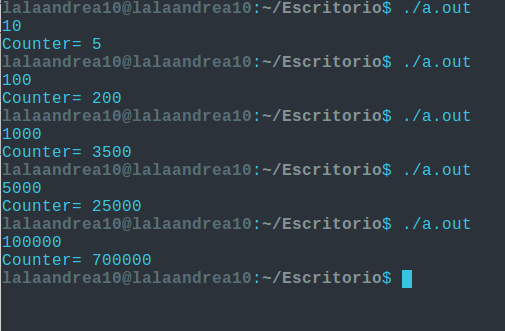
\includegraphics[scale=.5]{7P.png}
            \end{figure}
    \subsection{Algoritmo 8:}
    \lstinputlisting[language=C]{8.c}
    La respuesta en ninguna pues primero declaramos i=n y despues en el inicio del for j=n pero la condicino es que i<j pero esto nunca es cierto pues son iguales, entonces el while se seguira cumpliendo pero nunca entra.
    \section{Caso mejor, peor y medio.}
    \subsection{Algoritmo 9:}
    \lstinputlisting[language=C]{9.c}
    Analicemos por bloques:

    El primer if consta de una comparacio, y 2 asignaciones.

    Si no entra al if entonces tenemos que hacer la comparacion del if  y 2 instrucciones.

    Tenemos la asignacion que siempre se realiza.

    Curiosamente nos cuesta lo mismo elejir uno u otro.

    el while hará $n-2$ repeticiones de una compraracion.


    Además tenemos dentro el while tenemos un if que consta de 3 instrucciones.


    Ademas si entra tambien al segundo  la primera comparación, mas la compraracion y la asignacion.

    Tenemos 2 instrucciones dentro del while.

    Regresa una operación.

    \subsubsection{Mejor caso}
    Es cuando los 2 primeros son el mayor y el segundo mayor de esta manera tenemos 3 instrucciones antes del while, y $2(n-2)$  instrucciones dentro del while. 

    Por tnto la complejidad es $2n-1$

    \subsubsection{Peor Caso}
    Cuando el arreglo esta ordenado de menor a mayor.

    Tendremos 3 instrucciones iniciales y tendremos $3(n-2)$ dentro del while.

    Por lo tanto la coplejidad será de $3n-3$

    \subsubsection{Caso medio}
    Tenemos al inicio 3 instrucciones, de ahi se deriva el caso de que entre al primer if dentro del while, sería igual a $3n-3$ con el segundo es igual y si no entramos sería $2n-1$

    Entonces el caso medio será igual a :

    $\dfrac{1}{3}(3n-3)+\dfrac{1}{3}(3n-3)+\dfrac{1}{3}(2n-1)+3 = \dfrac{8n-7}{3}+3$

    \subsection{Algoritmo 10:}
    \lstinputlisting[language=C]{10.c}
    El if ejecuta 4 instrucciones. Si no se ejecuta es 1 instruccion.


    El for interno se ejecuta n-i-1 veces.

    El otro for se ejecuta n-1 veces.
    \subsubsection{Mejor caso}
    Cuando el arreglo esta ordenado ascendentemente.

    El if  no estra entonces tenemos una instrucción.
    La complejidad sería$ n^{2}+2n+1$

    \subsubsection{Peor caso}
    Cuando el arreglo esta descendentemente.
    El peor caso es 4 veces la del mejor caso.

    $4n^{2} +8n+4$

    \subsubsection{Caso medio}
    En este caso es el promedio del peor y el mejor caso entonces sería:
    $\dfrac{5n^{2}+10n+5}{2}$

    \subsection{Algoritmo 11:}
    \lstinputlisting[language=C]{11.c}
    \subsubsection{Mejor caso}

    Cuando n=0 nunca entramos al while entonces la complejidad es 0.

    \subsubsection{Peor caso}
    Entrara al while a/b. veces.
    Entonces asumiendo que n es el mayor y $m<<n$ entonces será n.

    \subsubsection{Caso medio}
    Sera el peor caso. n.
    \subsection{Algoritmo 12:}
    \lstinputlisting[language=C]{12.c}
    \subsubsection{Mejor caso}
    Cuando A esta ordenado ascendentemente.
    Entrara al while solo una vez y la varicable quea en No. Entonces será $n-1$

    \subsubsection{Peor caso}
    Cuando A esta ordenado descendentemente.

    En el while habra cambio en la variable entonces la complejidad será $n^{2}+2n+2$

    \subsubsection{Caso medio}
    La complejidad sera dependiendo del if.
    $\dfrac{2n^2-n-1}{2}$

    \subsection{Algoritmo 13:}
    \lstinputlisting[language=C]{13.c}
    El if ejecuta 4 instrucciones.
    Si no entra al if se ejecuta solo una.

    El for de más dentro se ejcuta n-i-1 veces y el mas fuera se ejecuta n-1 veces.

    \subsubsection{Mejor caso}
    Cuando el arreglo está ascendente.
    $\sum_{i=0}^{n-2} 1 = \dfrac{n^{2}-n}{2}$

    \subsubsection{Peor caso}
    Cuando el arreglo esta ordenado descentemente. Como el if tiene 4 instrucciones entonces la complejidad es: $2n^2 -2$

    \subsubsection{Caso medio}
    Será: $=\dfrac{n^2-n}{4}+\dfrac{2n^2-2}{2}$

    \subsection{Algoritmo 14}
    \lstinputlisting[language=C]{14.c}
    Tenemos una serie de comparaciones.
    \subsubsection{Mejor caso}
    Cuando entra a la primera compraración pero no a la segunda, y cuando se entra al primer else y al segundo else.
    La complejidad en este caso es $=2$.
    \subsubsection{Peor caso}
    Cuando estra a algun otra de las 4 combinaciones es de $=3$

    \subsubsection{Caso medio}
    Es la probabilidad de cada caso que es $=\dfrac{8}{3}$

    \subsection{Algoritmo 15:}
    \lstinputlisting[language=C]{15.c}
    El for mas dentro se realiza $n-k-1$ veces, el if que esta dentro cuesta 1 instruccion.

    Tenemos  otro for que se realiza n-1 veces, despues del for hace 3 opeaciones 
en caso de que entre al if o no.

    \subsubsection{Mejor caso}
    Cuando el arreglo esta ordenado ascendentemente.

    Entonces: $\sum{k=0}^{n-2}(3+\sum{i=k+1}^{n-1}1)=(n+2)(n-1)-\dfrac{(n-2)(n-1)}{2}$
    \subsubsection{Peor caso}
    Cuando el arrego esta ordenado descendemente.
    Curiosamente es la misma complejidad aunque la condicion del if siempre se cumpla.
    Entonces es la misma complejidad:

    $=(n+2)(n-1)-\dfrac{(n-2)(n-1)}{2}$

    \subsubsection{Caso medio}
    Como el peor y el mejor caso es el mismo, el caso medio es $=(n+2)(n-1)-\dfrac{(n-2)(n-1)}{2}$






% ===============================================
% ========        BIBLIO      ===================
% ===============================================
%\begin{thebibliography}{10}

    
 %   \bibitem{CodeName3} 
  %      Francisco Ruiz, Fac. de Ciencias
   %     \textit{https://www.ctr.unican.es/asignaturas/is1/is1-t02-trans.pdf}. 

%\end{thebibliography}

\end{document}
